\documentclass[../../main.tex]{subfiles}

\begin{document}

\subsection{Abstract}

A generalized multilinear regression model, termed the Higher-Order Partial Least Squares (HOPLS) \cite{HOPLS}, is introduced with the aim to predict a tensor $\tensor{Y}$ from a tensor $\tensor{X}$ through projecting the data onto the latent space and performing regression on the corresponding latent variables. This method could be applied to a wide range of datasets. To solve the problem of predicting eye movement we get time series of frames passed through Convolutional Neural Network (CNN).

\subsection{Problem statement}

We are given a dataset, that consists of several videos with eye movements and its positions. Let $\tensor{X}$ is an output of CNN, $\tensor{Y}$ --- eye coordinate. Assume $\tensor{X} \in \mathbb{R}^{I_1 \times ... \times I_N}$ and $\tensor{Y} \in \mathbb{R}^{J_1 \times ... \times J_M}$. We assume $\tensor{X}$ is decomposed as a sum of rank-$(1,L_2,...,L_N)$ Tucker blocks, while $\tensor{Y}$ is decomposed as a sum of rank-$(1, K_2,...,K_M)$ Tucker blocks, which can be expressed as

\begin{equation}
    \begin{split}
        \tensor{X} = \sum_{r=1}^R \tensor{G}_r \times_1 \textbf{t}_r \times_2 \textbf{P}_r^{(1)} \times_3 ... \times_n \textbf{P}_r^{(n-1)} + \tensor{E}_R \\
        \tensor{Y} = \sum_{r=1}^R \tensor{D}_r \times_1 \textbf{t}_r \times_2 \textbf{Q}_r^{(1)} \times_3 ... \times_n \textbf{Q}_r^{(n-1)} + \tensor{F}_R
    \end{split}
\end{equation}

\begin{figure}[h!]
\centering
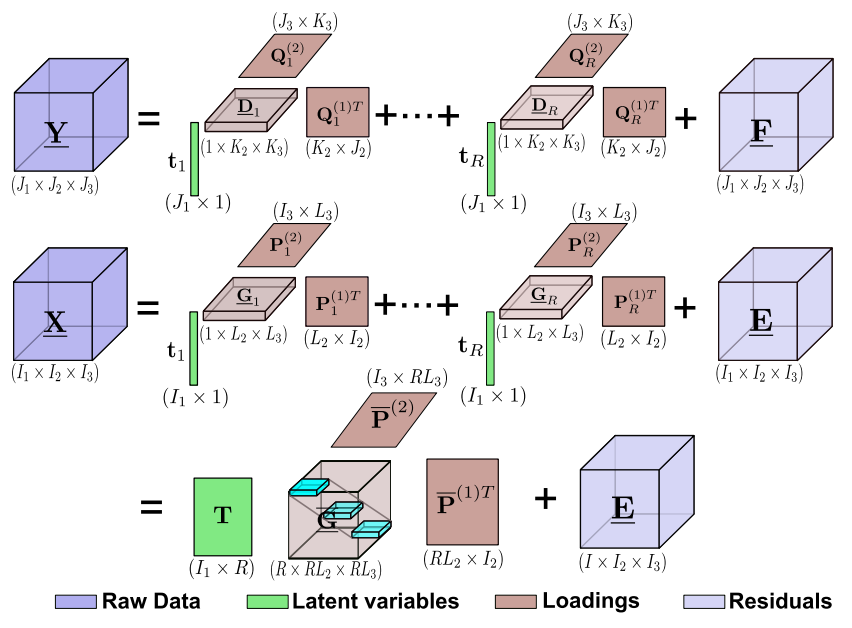
\includegraphics[width=0.8\textwidth]{figures/HOPLS}
\caption{Schematic diagram of the HOPLS model}
\label{fig:eye_pred:1}
\end{figure} 

\noindent where $R$ is the number of latent vectors, $t_r \in \mathbb{R}^{I_1}$ is the $r$-th latent vector, $\left\{\textbf{P}_r^{(n)}\right\}_{n=1}^{N-1} \in \mathbb{R}^{I_{n+1} \times L_{n+1}}$ and 
$\left\{\textbf{Q}_r^{(m)}\right\}_{m=1}^{M-1} \in \mathbb{R}^{J_{n+1} \times K_{n+1}}$
are loading matrices on mode-$n$ and mode-$m$ respectively, and $\tensor{G}_r \in \mathbb{R}^{1 \times L_2 \times ... \times L_N}$ and $\tensor{D}_r \in \mathbb{R}^{1 \times K_2 \times ... \times K_M}$ are core tensors.

To make a prediction we should use 
\begin{equation}
    \label{prediction}
    \hat{\tensor{Y}} = \tensor{X} \textbf{W} \textbf{Q}^{* \top}
\end{equation}
where $\textbf{W}$ and $\textbf{Q}^{*}$ have $R$ columns, represented by
\begin{equation}
    \begin{split}
        & \textbf{w}_r = \left( \textbf{P}_r^{(N-1)} \otimes ... \otimes \textbf{P}_r^{(1)} \right) \tensor{G}_{r}^+ \\
        & \textbf{q}^*_r = \tensor{D}_{r} \left( \textbf{Q}_r^{(M-1)} \otimes ... \otimes \textbf{Q}_r^{(1)} \right)
    \end{split}
\end{equation}

\subsection{Problem solution}

Use CNN that converts 480x640 pixels images to 24x32 resolution. Its output is $\tensor{X}$. So $N = 3, I_2 = 34, I_3 = 39$. $\tensor{Y}$ tensor is given and it is 2 dimensional tensor with $J_2 = 2$ (Fig. \ref{fig:eye_pred:2}). For these tensors we use Higher-Order Partial Least Squares algorithm described in \cite{HOPLS} and make a prediction according \eqref{prediction}. 

\begin{figure}[h!]
\centering
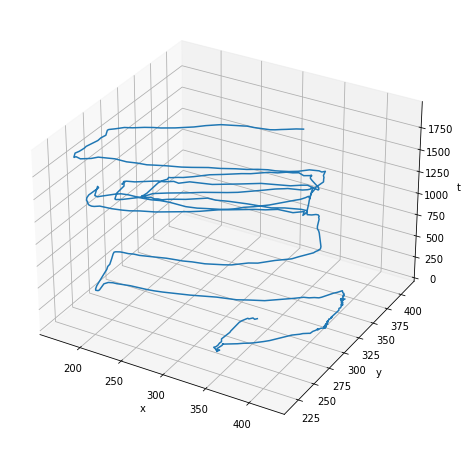
\includegraphics[width=0.8\textwidth]{figures/trajectory}
\caption{Trajectory of the center of eye}
\label{fig:eye_pred:2}
\end{figure}

\subsection{Code}

HOPLS algorithm was made by Arthur Dehgan, co-author of \cite{HOPLS} and avalible at  https://github.com/arthurdehgan/HOPLS.
The code for computation experiment is located on https://github.com/artem062/ForecastingMethods.

\subsection{Experiment}

It was used LPW dataset, that consist of 66 videos with eye moving. This videos was compressed and converted to the tensors. To archive the best $R$ plot the value of $Q^2 = 1 - \|\tensor{Y} - \hat{\tensor{Y}}\|^2_F / \|\tensor{Y}\|^2_F$.

\begin{figure}[h!]
\centering
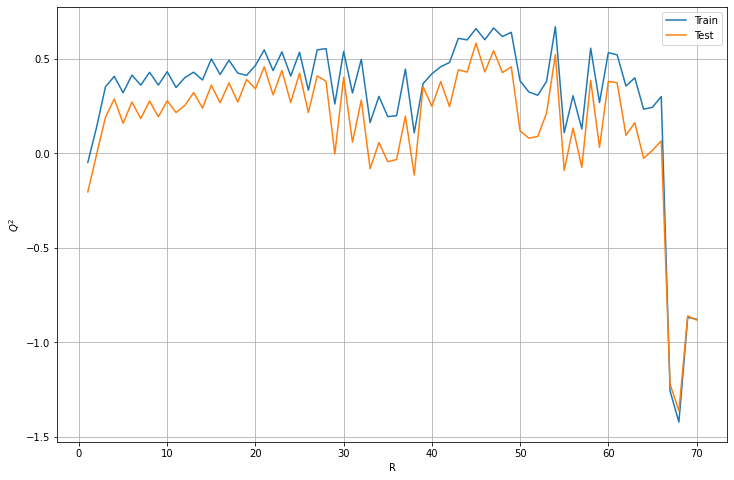
\includegraphics[width=1.0\textwidth]{figures/plot}
\caption{Graph of dependence of $Q^2$ on $R$}
\label{fig:eye_pred:3}
\end{figure}

This graph shows that optimal value of $R$ by train dataset is 54, but for test it is 45.

\end{document}